\documentclass[10pt,
  aspectratio=169,
  serif,
  mathserif,
  professionalfont,
  compress,
  handout,
  % table,
  % svgnames
  ]{beamer}\usepackage[]{graphicx}\usepackage[]{color}
% maxwidth is the original width if it is less than linewidth
% otherwise use linewidth (to make sure the graphics do not exceed the margin)
\makeatletter
\def\maxwidth{ %
  \ifdim\Gin@nat@width>\linewidth
    \linewidth
  \else
    \Gin@nat@width
  \fi
}
\makeatother

\definecolor{fgcolor}{rgb}{1, 1, 0.941}
\newcommand{\hlnum}[1]{\textcolor[rgb]{0.804,0.718,0.71}{#1}}%
\newcommand{\hlstr}[1]{\textcolor[rgb]{0.604,0.753,0.804}{#1}}%
\newcommand{\hlcom}[1]{\textcolor[rgb]{0.439,0.502,0.565}{#1}}%
\newcommand{\hlopt}[1]{\textcolor[rgb]{1,1,0.941}{#1}}%
\newcommand{\hlstd}[1]{\textcolor[rgb]{1,1,0.941}{#1}}%
\newcommand{\hlkwa}[1]{\textcolor[rgb]{0.941,0.902,0.549}{#1}}%
\newcommand{\hlkwb}[1]{\textcolor[rgb]{1,0.871,0.678}{#1}}%
\newcommand{\hlkwc}[1]{\textcolor[rgb]{0.545,0.941,0.702}{#1}}%
\newcommand{\hlkwd}[1]{\textcolor[rgb]{0.545,0.941,0.902}{#1}}%
\let\hlipl\hlkwb

\usepackage{framed}
\makeatletter
\newenvironment{kframe}{%
 \def\at@end@of@kframe{}%
 \ifinner\ifhmode%
  \def\at@end@of@kframe{\end{minipage}}%
  \begin{minipage}{\columnwidth}%
 \fi\fi%
 \def\FrameCommand##1{\hskip\@totalleftmargin \hskip-\fboxsep
 \colorbox{shadecolor}{##1}\hskip-\fboxsep
     % There is no \\@totalrightmargin, so:
     \hskip-\linewidth \hskip-\@totalleftmargin \hskip\columnwidth}%
 \MakeFramed {\advance\hsize-\width
   \@totalleftmargin\z@ \linewidth\hsize
   \@setminipage}}%
 {\par\unskip\endMakeFramed%
 \at@end@of@kframe}
\makeatother

\definecolor{shadecolor}{rgb}{.97, .97, .97}
\definecolor{messagecolor}{rgb}{0, 0, 0}
\definecolor{warningcolor}{rgb}{1, 0, 1}
\definecolor{errorcolor}{rgb}{1, 0, 0}
\newenvironment{knitrout}{}{} % an empty environment to be redefined in TeX

\usepackage{alltt}

% Tamanho de fonte e distância entre linhas.
\renewenvironment{knitrout}{
  \renewcommand{\baselinestretch}{0.75}%\tiny
}{}

%-----------------------------------------------------------------------
% Pacotes padrões.

% Fontes.
\usepackage{palatino}
\usepackage{eulervm}
\usepackage{inconsolata}

% Esses pacotes dão clash.
% http://tex.stackexchange.com/questions/51488/option-clash-with-xcolor-and-tikz
% \usepackage{xcolor} %% opções no \documentclass{} para evitar clash.
% \definecolor{mycolor}{rgb}{0.13,0.53,0.53}
% \definecolor{mycolor2}{rgb}{0.725,0,0.18}

\usepackage{hyperref}
 \hypersetup{colorlinks, allcolors=., urlcolor=structure}
% \hypersetup{colorlinks}

\usepackage[brazil]{babel}
\usepackage[utf8]{inputenc}
\usepackage{graphicx}
\usepackage{amsmath, amsfonts, amssymb, amsxtra, amsthm, icomma}
\usepackage{geometry, calc, setspace, indentfirst}
% \usepackage{colortbl}
\usepackage{enumerate}
\usepackage{float}

\usepackage{subfigure}

\usepackage[hang]{caption}
\captionsetup{font=footnotesize,
  labelfont=footnotesize,
  labelsep=period}

% Listas em duas colulas.
\usepackage{multicol}
\newenvironment{itemize2}{%
  \vspace*{-1em}
  \begin{itemize}
    \begin{multicols}{2}
    }{%
    \end{multicols}
  \end{itemize}
}

% Texto no corpo do beamer justificado.
\usepackage{ragged2e}
\justifying

%-----------------------------------------------------------------------

% A lot of options:
% http://latex-community.org/forum/viewtopic.php?f=55&t=17646
\useoutertheme[
  width=60pt,
  height=30pt,
  right,
  hideothersubsections
  ]{sidebar}

\makeatletter
\setbeamertemplate{caption}[numbered]
\setbeamertemplate{section in toc}[sections numbered]
\setbeamertemplate{subsection in toc}[subsections numbered]
\setbeamertemplate{sections/subsections in toc}[ball]{}
\setbeamertemplate{section in sidebar right}[sections numbered]
%\setbeamertemplate{frametitle continuation}{\gdef\beamer@frametitle{}}
\setbeamertemplate{navigation symbols}{} %% Retira a barra de navegação.
% \setbeamertemplate{blocks}[rounded][shadow=FALSE]
% \setbeamercolor{block title}{fg=structure, bg=mycolor!20!white}
\makeatother

% Frames com sessão e/ou subsessão.
% \addtobeamertemplate{frametitle}{
%   \let\insertframetitle\insertsubsectionhead}{}
% \makeatletter
% \CheckCommand*\beamer@checkframetitle{
%   \@ifnextchar\bgroup\beamer@inlineframetitle{}}
% \renewcommand*\beamer@checkframetitle{
%   \global\let\beamer@frametitle\relax\@ifnextchar\bgroup
%   \beamer@inlineframetitle{}}
% \makeatother

\setbeamertemplate{frametitle}
{
    \nointerlineskip
    \begin{beamercolorbox}[sep=0.3cm,ht=1.8em,wd=\paperwidth]{frametitle}
        \vbox{}\vskip-2ex%
        \strut\insertframetitle\strut
        \vskip-0.8ex%
    \end{beamercolorbox}
}


%-----------------------------------------------------------------------
% Comandos.

\newcommand{\n}[1]{\textbf{#1}}

%-----------------------------------------------------------------------

\AtBeginSection[]{
  \begin{frame}[c,allowframebreaks]
    \begin{center}
      {\thesection} \\ \vspace{0.3cm}
      \parbox{0.6\textwidth}{
        \centering {\Large \textcolor{structure}{\insertsection}}}\\
    \end{center}
  \end{frame}
}

%-----------------------------------------------------------------------
% Definições dos proprietários.

\title[TH MCGLM]{
  \LARGE Testes de hipótese em Modelos\\  Multivariados de Covariância  \\ Linear Generalizada (McGLM)}


\author[Lineu Alberto]{%\small
  Lineu Alberto Cavazani de Freitas \\
  Orientador: Prof. Dr. Wagner Hugo Bonat
}

\institute[UFPR]{
  PPG Informática \\
  Data Science \& Big Data \\
  Universidade Federal do Paraná\\

  \vspace{1em}
  \href{}{https://lineu96.github.io/st/}\\
  \texttt{lineuacf@gmail.com}
}
\date{}

\logo{
\includegraphics[width=1.5cm]{img/dsbd1x4-rect.png}} 

\usebackgroundtemplate{
  
\includegraphics[width=\paperwidth]{img/ufpr-fundo.jpg}
}

%=======================================================================
%=======================================================================
\IfFileExists{upquote.sty}{\usepackage{upquote}}{}
\begin{document}

\frame{\titlepage}

% Tabela de conteúdo no início dos slides.
% \begin{frame}{Conteúdo}
%   \small{\tableofcontents}
% \end{frame}

%-----------------------------------------------------------------------



% -----------------------------------------------------------------

\section{Quem sou eu}

% -----------------------------------------------------------------

\begin{frame}

\begin{columns}
\begin{column}{0.7\textwidth}
   
   \textbf{Quem sou eu}
   
   \begin{itemize}

  \item Estatístico formado pela \href{https://www.ufpr.br/portalufpr/}{Universidade Federal do Paraná (UFPR)} em 2019.

  \item Atualmente mestrando no \href{http://www.prppg.ufpr.br/ppginformatica/?lang=pb}{Programa de Pós Graduação em Informática da UFPR}.
  
  \item Inserido na área de concentração Ciência da Computação, linha de pesquisa Tecnologia da Informação e grupo de pesquisa \href{https://web.inf.ufpr.br/dsbd/}{Data Science \& Big Data}.
  
  \end{itemize}
  
\end{column}
\begin{column}{0.3\textwidth}  %%<--- here
    \begin{center}
     
\includegraphics[width=\textwidth]{img/eu3.jpeg}
     \end{center}
\end{column}
\end{columns}
\end{frame}

% -----------------------------------------------------------------

\begin{frame}[c, allowframebreaks]
  
  \textbf{Sumário}
  
  \begin{enumerate}
  
    \item Introdução
    
    \item McGLM
    
    \item Estimação e inferência
    
    \item Teste Wald
    
    \item Construção da matriz L
    
    \item ANOVA via teste Wald
    
    \item Funções implementadas
    
    \item Próximos passos
    
  \end{enumerate}

\end{frame}

% -----------------------------------------------------------------

\section{Introdução}

\begin{frame}[c, allowframebreaks]
  
  \textbf{Onde tudo começou}
  
  \begin{itemize}

  \item O projeto teve início em 2018 quando eu e uma colega de curso (\href{https://br.linkedin.com/in/jhecaetano}{Jhenifer Caetano Veloso}), desenvolvemos nosso TCC sob orientação do professor Wagner. 

  \item O título do trabalho foi "\href{https://lineu96.github.io/st/projects/manova/}{Análise de Variância Multivariada para Dados Não Gaussianos via Teste Wald}".
  
  \end{itemize}

\end{frame}

% -----------------------------------------------------------------

\begin{frame}[c, allowframebreaks]

\begin{center}  
  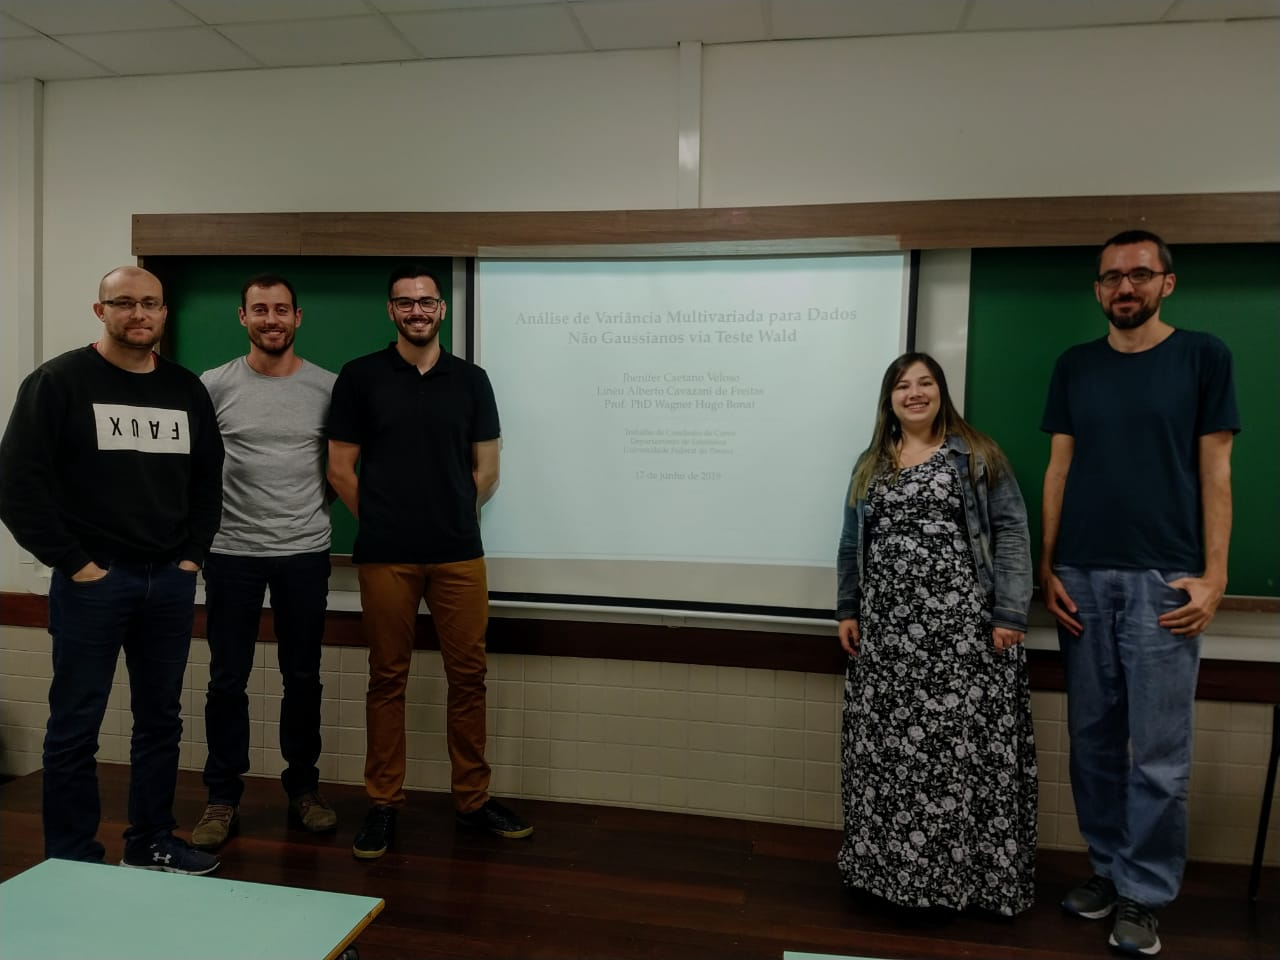
\includegraphics[width=9.4cm]{img/tcc.jpg}  
\end{center}

\end{frame}

\begin{frame}[c, allowframebreaks]
  
  \textbf{Plano para o mestrado}
  
  \begin{itemize}
  
  \item Na graduação avaliamos o teste Wald para gerar quadros de análise de variância multivariadas do tipo III (MANOVA).
  
  \item A ideia é dar continuidade e ampliar o foco do trabalho que teve início na graduação.
  
  \item O título atual do trabalho é "Testes de hipótese em Modelos Multivariados de Covariância Linear Generalizada (McGLM)".

  \item Nosso objetivo é explorar o teste Wald para testar hipóteses gerais sobre parâmetros de regressão, dispersão ou potência de um McGLM.
  
  \item Bem como obter quadros de ANOVA e MANOVA para parâmetros de regressão e dispersão.

  \end{itemize}

\end{frame}

% -----------------------------------------------------------------

\begin{frame}[c, allowframebreaks]
  
  \textbf{As etapas do trabalho são:}
  
  \begin{itemize}
    \item Adaptar o teste Wald para realização de testes de hipótese gerais sobre parâmetros de Modelos Multivariados de Covariância Linear Generalizada (McGLM).
    
    \item Implementar funções para efetuar tais testes, bem como funções para efetuar Análises de Variância e Análises de Variância Multivariadas para os McGLM.
    
    \item Demonstrar as propriedades e comportamento dos testes propostos com base em estudos de simulação.
    
    \item Demonstrar o potencial de aplicação das metodologias discutidas com base na aplicação a conjuntos de dados reais.
    
  \end{itemize}

\end{frame}

% -----------------------------------------------------------------

\section{McGLM}

\begin{frame}[c, allowframebreaks]

\textbf{Para definição de um McGLM considere:}

\begin{itemize}
  
  \item $\boldsymbol{Y}_{N \times R} = \left \{ \boldsymbol{Y}_1, \dots, \boldsymbol{Y}_R \right \}$ uma  matriz de variáveis resposta.
  
  \item $\boldsymbol{M}_{N \times R} = \left \{ \boldsymbol{\mu}_1, \dots, \boldsymbol{\mu}_R \right \}$ uma matriz de valores esperados.
  
  \item $\Sigma_r$, $r = 1,..., R$, a matriz de variância e covariância para cada resposta $r$, de dimensão $NxN$.
  
  \item $\Sigma_b$ uma matriz de correlação, de ordem $R \times R$, que descreve a correlação entre as variáveis resposta.
  
    \item $\boldsymbol{X}_r$ denota uma matriz de delineamento $N \times k_r$.
  
  \item $\boldsymbol{\beta}_r$ denota um vetor $k_r \times 1$ de parâmetros de regressão.
  
\end{itemize}

\end{frame}

% -----------------------------------------------------------------

\begin{frame}[c, allowframebreaks]

\textbf{Os McGLMs são definidos por:}

\begin{center}
$\mathrm{E}(\boldsymbol{Y}) = \boldsymbol{M} = \{g_1^{-1}(\boldsymbol{X}_1 \boldsymbol{\beta}_1), \ldots, g_R^{-1}(\boldsymbol{X}_R \boldsymbol{\beta}_R)\}$

$\mathrm{Var}(\boldsymbol{Y}) = \boldsymbol{C} = \boldsymbol{\Sigma}_R \overset{G} \otimes \boldsymbol{\Sigma}_b$

\end{center}
    
Em que: 

\begin{itemize}
  
  \item $\boldsymbol{\Sigma}_R \overset{G} \otimes \boldsymbol{\Sigma}_b = \mathrm{Bdiag}(\tilde{\boldsymbol{\Sigma}}_1, \ldots, \tilde{\boldsymbol{\Sigma}}_R) (\boldsymbol{\Sigma}_b \otimes \boldsymbol{I}) \mathrm{Bdiag}(\tilde{\boldsymbol{\Sigma}}_1^\top, \ldots, \tilde{\boldsymbol{\Sigma}}_R^\top)$ é o produto generalizado de Kronecker.
  
  \item $\tilde{\boldsymbol{\Sigma}}_r$ denota a matriz triangular inferior da decomposição de Cholesky da matriz ${\boldsymbol{\Sigma}}_r$.
  
  \item $\mathrm{Bdiag()}$ denota a matriz bloco-diagonal.
  
  \item $\boldsymbol{I}$ uma matriz identidade $N \times N$.
  
  \item $g_r()$ são as tradicionais funções de ligação.
  
\end{itemize}

\end{frame}

% -----------------------------------------------------------------

\begin{frame}[c, allowframebreaks]

\textbf{Matriz de variância e covariância}

\begin{itemize}

  \item Para variáveis resposta contínuas, binárias, binomiais, proporções ou índices a matriz de variância e covariância $\boldsymbol{\Sigma}_r$ é dada por:
  
$$
\Sigma_r = \mathrm{V}\left(\boldsymbol{\mu}_r; p_r\right)^{1/2}(\boldsymbol{\Omega}\left(\boldsymbol{\tau}_r\right))\mathrm{V}\left(\boldsymbol{\mu}_r; p_r\right)^{1/2}
$$

  \item No caso de variáveis resposta que sejam contagens a matriz de variância e covariância para cada variável resposta fica dada por:

$$
\Sigma_r = diag(\boldsymbol{\mu}_r)+ \mathrm{V}\left(\boldsymbol{\mu}_r; p_r\right)^{1/2}(\boldsymbol{\Omega}\left(\boldsymbol{\tau}_r\right))\mathrm{V}\left(\boldsymbol{\mu}_r; p_r\right)^{1/2}
$$

  \item $\mathrm{V}\left(\boldsymbol{\mu}_r; p_r\right) = diag(\vartheta(\boldsymbol{\mu}_r; p_r))$ denota uma matriz diagonal na qual as entradas são dadas pela função de variância $\vartheta(\cdot; p_r)$ aplicada aos elementos do vetor $\boldsymbol{\mu}_r$.
  
\end{itemize}

\end{frame}

% -----------------------------------------------------------------

\begin{frame}[c, allowframebreaks]

\textbf{Função de variância}

\begin{itemize}
  
  \item Função de variância potência: 
  
  \begin{itemize}
    
    \item Caracteriza a família Tweedie de distribuições. 
    
    \item É dada por $\vartheta\left(\cdot; p_r\right) = \mu^{p_r}_r$.
    
    \item Casos particulares: Normal ($p$ = 0), Poisson ($p$ = 1), gama ($p$ = 2) e  Normal inversa ($p$ = 3).
    
  \end{itemize}
  
  \item Função de dispersão Poisson–Tweedie:
  
  \begin{itemize}
    
    \item Visa contornar a inflexibilidade da utilização da função de variância potência para respostas que caracterizam contagens. 
    
    \item É dada por $\vartheta\left(\cdot; p\right) = \mu + \tau\mu^p$ em que $\tau$ é o parâmetro de dispersão.
    
    \item Casos particulares: Hermite ($p$ = 0), Neyman tipo A ($p$ = 1), binomial negativa ($p$ = 2) e Poisson–inversa gaussiana (p = $3$).
  
  \end{itemize}

  \item Função de variância binomial: 
  
  \begin{itemize}
    
    \item Indicada quando a variável resposta é binária, restrita a um intervalo ou quando tem-se o número de sucessos em um número de tentativas.
    
    \item É dada por $\vartheta\left(\cdot; p_r\right) = \mu^{p_{r1}}_r(1 - \mu_r)^{p_{r2}}$ 
    
  \end{itemize}

  
\end{itemize}


\end{frame}

% -----------------------------------------------------------------

\begin{frame}[c, allowframebreaks]

\textbf{Parâmetro de potência}

\begin{itemize}
  
  \item O parâmetro de potência $p$ aparece em todas as funções de variância discutidas.
  
  \item Este parâmetro tem especial importância pois trata-se de um índice que distingue diferentes distribuições de probabilidade.
  
  \item Pode ser utilizado como uma ferramenta para seleção automática da distribuição de probabilidade que mais se adequa ao problema.
  
\end{itemize}

\end{frame}

% -----------------------------------------------------------------

\begin{frame}[c, allowframebreaks]

\textbf{Preditor linear matricial}

\begin{itemize}
  
  \item A matriz de dispersão $\boldsymbol{\Omega({\tau})}$ descreve a parte da covariância dentro de cada variável resposta que não depende da estrutura média. 
  
  \item Isto é, a estrutura de correlação entre as observações da amostra.
  
  \item A matriz de dispersão é modelada através de um preditor linear matricial combinado com uma função de ligação de covariância.
  
  \item O preditor linear matricial é dado por:

$$
h\left \{ \boldsymbol{\Omega}(\boldsymbol{\tau}_r) \right \} = \tau_{r0}Z_0 + \ldots + \tau_{rD}Z_D
$$
  
  \begin{itemize}
  
  \item $h()$ é a função de ligação de covariância.
  
  \item $Z_{rd}$ com $d$ = 0,$\ldots$, D são matrizes que representam a estrutura de covariância presente em cada variável resposta $r$.
  
  \item $\boldsymbol{\tau_r}$ = $(\tau_{r0}, \ldots, \tau_{rD})$ é um vetor $(D + 1) \times 1$ de parâmetros de dispersão. 
  
\end{itemize}

     
\end{itemize}

\end{frame}

% -----------------------------------------------------------------

\begin{frame}[c, allowframebreaks]

\textbf{Comentários sobre a classe}

\begin{itemize}
  
  \item Os McGLM configuram uma estrutura geral para análise via modelos de regressão.
  
  \item Comporta múltiplas respostas não gaussianas.
  
  \item Não se faz suposições quanto à independência das observações. 
  
\end{itemize}

\end{frame}

% -----------------------------------------------------------------

\section{Estimação e inferência}

\begin{frame}[c, allowframebreaks]

\textbf{Funções de estimação}

As funções de estimação para os parâmetros de regressão (função quasi-score) e de dispersão (função de estimação de Pearson) são dadas por:

\begin{center}
$\psi_{\boldsymbol{\beta}}(\boldsymbol{\beta}, \boldsymbol{\lambda}) = \boldsymbol{D}^\top \boldsymbol{C}^{-1}(\mathcal{Y} - \mathcal{M})$

$\psi_{\boldsymbol{\lambda}_i}(\boldsymbol{\beta}, \boldsymbol{\lambda}) = \mathrm{tr}(W_{\boldsymbol{\lambda}i} (\boldsymbol{r}^\top\boldsymbol{r} - \boldsymbol{C})),  i = 1,.., Q$
\end{center}

Em que:

\begin{itemize}
  
  \item $\boldsymbol{\beta}_r$ denota um vetor $k_r \times 1$ de parâmetros de regressão.
  
  \item $\boldsymbol{\lambda}$ é um vetor $Q \times 1$ de parâmetros de dispersão.
  
  \item $\mathcal{Y}$ é um vetor $NR \times 1$ com os valores da matriz de variáveis respostas $Y_{N \times R}$ empilhados.
  
  \item $\mathcal{M}$ é um vetor $NR \times 1$ com os valores da matriz de valores esperados $M_{N \times R}$ empilhados.
  
  \item $\boldsymbol{D} = \nabla_{\boldsymbol{\beta}} \mathcal{M}$ 
é uma matriz $NR \times K$, e $\nabla_{\boldsymbol{\beta}}$ denota o 
operador gradiente.
  
  \item $W_{\boldsymbol{\lambda}i} = -\frac{\partial
    \boldsymbol{C}^{-1}}{\partial \boldsymbol{\lambda}_i}$ 
    
  \item $\boldsymbol{r} = (\mathcal{Y} - \mathcal{M})$
  
\end{itemize}

\end{frame}

% -----------------------------------------------------------------

\begin{frame}[c, allowframebreaks]

\textbf{Distribuição assintótica e algoritmo de estimação}

\begin{itemize}

  \item Para resolver o sistema de equações $\psi_{\boldsymbol{\beta}} = 0$ e $\psi_{\boldsymbol{\lambda}} = 0$ faz-se uso do algoritmo Chaser modificado:

$$
\begin{matrix}
\boldsymbol{\beta}^{(i+1)} = \boldsymbol{\beta}^{(i)}- S_{\boldsymbol{\beta}}^{-1} \psi \boldsymbol{\beta} (\boldsymbol{\beta}^{(i)}, \boldsymbol{\lambda}^{(i)}), \\ 
\boldsymbol{\lambda}^{(i+1)} = \boldsymbol{\lambda}^{(i)}\alpha S_{\boldsymbol{\lambda}}^{-1} \psi \boldsymbol{\lambda} (\boldsymbol{\beta}^{(i+1)}, \boldsymbol{\lambda}^{(i)}).
\end{matrix}
$$

  \item Seja $\boldsymbol{\hat{\theta}} = (\boldsymbol{\hat{\beta}^{\top}}, \boldsymbol{\hat{\lambda}^{\top}})^{\top}$ o estimador baseado em funções de estimação de $\boldsymbol{\theta}$.
  
  \item A distribuição assintótica de $\boldsymbol{\hat{\theta}}$ é:

$$
\boldsymbol{\hat{\theta}} \sim N(\boldsymbol{\theta}, J_{\boldsymbol{\theta}}^{-1}),
$$

\noindent $J_{\boldsymbol{\theta}}^{-1}$ é a inversa da matriz de informação de Godambe, dada por
  
$$J_{\boldsymbol{\theta}}^{-1} = S_{\boldsymbol{\theta}}^{-1} V_{\boldsymbol{\theta}} S_{\boldsymbol{\theta}}^{-\top},$$ 

\noindent em que $S_{\boldsymbol{\theta}}^{-\top} = (S_{\boldsymbol{\theta}}^{-1})^{\top}.$

\end{itemize}

\end{frame}

% -----------------------------------------------------------------

\section{Teste Wald}

\begin{frame}[c, allowframebreaks]

\textbf{Teste Wald}

\begin{itemize}
  
  \item E um teste de hipóteses largamente empregado para avaliar suposições sobre parâmetros de um modelo de regressão.
  
  \item Isto é, verifcar se existe evidência suficiente para afirmar que o parâmetro é ou não estatísticamente igual a um valor qualquer. 
  
\end{itemize}

\end{frame}

% -----------------------------------------------------------------

\begin{frame}[c, allowframebreaks]

\textbf{Teste Wald}

\begin{itemize}

  \item A grosso modo, é um teste que avalia a distância entre a estimativa do parâmetro e o valor postulado sob a hipótese nula. 
  
  \item Esta diferença é ainda ponderada por uma medida de precisão da estimativa do parâmetro. 
  
  \item Quanto mais distante de 0 for o valor da distância ponderada, menor é a chance da hipótese de igualdade ser verdadeira, ou seja, do valor postulado ser igual ao valor estimado. 

\end{itemize}

\end{frame}

% -----------------------------------------------------------------

\begin{frame}[c, allowframebreaks]

\textbf{Teste Wald}

\begin{itemize}

\item Além destes elementos o teste pressupõe que os estimadores dos parâmetros do modelo sigam distribuição assintótica Normal.

\item Para avaliação da estatística de teste e verificação de significância estatística utiliza-se distribuição assintótica Qui-quadrado ( $\chi^2$ ).

\end{itemize}

\end{frame}

% -----------------------------------------------------------------

\begin{frame}[c, allowframebreaks]

\textbf{Hipóteses}

As hipóteses a serem testadas podem ser escritas como:

$$H_0: \boldsymbol{L}\boldsymbol{\theta_{\beta,\tau,p}} = \boldsymbol{c} \ vs \ H_1: \boldsymbol{L}\boldsymbol{\theta_{\beta,\tau,p}} \neq \boldsymbol{c}.$$ 

Em que: 

\begin{itemize}
  
  \item Em que $\boldsymbol{L}$ é a matriz de especificação das hipóteses a serem testadas, tem dimensão $s \times h$. 
  
  \item $\boldsymbol{\theta_{\beta,\tau,p}}$ é o vetor de dimensão $h \times 1$ de parâmetros de regressão, dispersão e potência do modelo. 
  
  \item $\boldsymbol{c}$ é um vetor de dimensão $s \times 1$ com os valores sob hipótese nula.

\end{itemize}

\end{frame}

% -----------------------------------------------------------------

\begin{frame}[c, allowframebreaks]

\textbf{Estatística de teste}

A generalização da estatística de teste para verificar a validade de uma hipótese sobre parâmetros de um McGLM é dada por:

$$W = (\boldsymbol{L\hat\theta_{\beta,\tau,p}} - \boldsymbol{c})^T \ (\boldsymbol{L \ J_{\boldsymbol{{\beta,\tau,p}}}^{-1} \ L^T})^{-1} \ (\boldsymbol{L\hat\theta_{\beta,\tau,p}} - \boldsymbol{c}).$$

Em que: 

\begin{itemize}
  \item $\boldsymbol{L}$ é a mesma matriz da especificação das hipóteses a serem testadas, tem dimensão $s \times h$. 

  \item $\boldsymbol{\hat\theta_{\beta,\tau,p}}$ é o vetor de dimensão $h \times 1$ com todas as estimativas dos parâmetros de regressão, dispersão e potência do modelo. 

  \item $\boldsymbol{c}$ é um vetor de dimensão $s \times 1$ com os valores sob hipótese nula. 

  \item E $J_{\boldsymbol{{\beta,\tau,p}}}^{-1}$ é a inversa da matriz de informação de Godambe desconsiderando os parâmetros de correlação, de dimensão $h \times h$. 

\end{itemize}

\end{frame}

% -----------------------------------------------------------------

\begin{frame}[c, allowframebreaks]

\textbf{A matriz \textbf{L}}

\begin{itemize}
  
  \item Cada coluna da matriz $\boldsymbol{L}$ corresponde a um dos $h$ parâmetros do modelo e cada linha a uma hipótese. 
  
  \item Sua construção consiste basicamente em preencher a matriz com 0, 1 e eventualmente -1 de tal modo que o produto $\boldsymbol{L}\boldsymbol{\theta_{\beta,\tau,p}}$ represente corretamente a hipótese de interesse.
  
\end{itemize}

\end{frame}

% -----------------------------------------------------------------

\begin{frame}[c, allowframebreaks]

\textbf{Comentários finais}

\begin{itemize}
  
  \item É possível testar qualquer parâmetro individualmente ou até mesmo formular hipóteses para diversos parâmetros simultaneamente, sejam eles de regressão, dispersão ou potência. 
  
  \item Independente do número de parâmetros testados, a estatística de teste $W$ é um único valor que segue assintóticamente distribuição $\chi^2$.
  
  \item Os graus de liberdade são dados pelo número de parâmetros testados, isto é, o número de linhas da matriz $\boldsymbol{L}$, denotado por $s$.
  
\end{itemize}

\end{frame}

% -----------------------------------------------------------------

\section{Construção da matriz L}

\begin{frame}[c, allowframebreaks]

\textbf{Exemplos de hipóteses que podem ser testadas.}

Considere um modelo bivariado genérico, com preditor dado por:

$$g_r(\mu_r) = \beta_{r0} + \beta_{r1} x_1$$

\begin{itemize}
  
  \item O índice $r$ denota a variável resposta, r = 1,2.
  
  \item $\beta_{r0}$ representa o intercepto.
  
  \item $\beta_{r1}$ um parâmetro de regressão associado a uma variável $x_1$.
  
  \item Considere que cada resposta possui apenas um parâmetro de dispersão: $\tau_{r1}$.
  
  \item Considere que os parâmetros de potência foram fixados.
  
\end{itemize}

\end{frame}

% -----------------------------------------------------------------

\begin{frame}[c, allowframebreaks]

\textbf{Exemplo 1}

Considere a hipótese:

$$H_0: \beta_{11} = 0 \ vs \ H_1: \beta_{11} \neq 0.$$

Esta hipótese pode ser reescrita na seguinte notação:

$$H_0: \boldsymbol{L}\boldsymbol{\theta_{\beta,\tau,p}} = \boldsymbol{c} \ vs \ H_1: \boldsymbol{L}\boldsymbol{\theta_{\beta,\tau,p}} \neq \boldsymbol{c}.$$ 

Em que:

\begin{itemize}
  
  \item $\boldsymbol{\theta_{\beta,\tau,p}^T}$ = $\begin{bmatrix} \beta_{10} \  \beta_{11} \ \beta_{20} \ \beta_{21} \ \tau_{11} \ \tau_{21} \end{bmatrix}$.


\item $\boldsymbol{L} = \begin{bmatrix} 0 & 1 & 0 & 0 & 0 & 0  \end{bmatrix}.$
 
\item $\boldsymbol{c}$ = $\begin{bmatrix} 0 \end{bmatrix}$, é o valor da hipótese nula. 

\end{itemize}

\end{frame}

% -----------------------------------------------------------------

\begin{frame}[c, allowframebreaks]

\textbf{Exemplo 2}

Considere a hipótese:

$$H_0: \beta_{r1} = 0 \ vs \ H_1: \beta_{r1} \neq 0.$$ 

Ou, da mesma forma:

$$H_0: 
\begin{pmatrix}
\beta_{11} \\ 
\beta_{21}
\end{pmatrix} 
= 
\begin{pmatrix}
0 \\ 
0
\end{pmatrix}
\ vs \ 
H_1: 
\begin{pmatrix}
\beta_{11} \\ 
\beta_{21}
\end{pmatrix} 
\neq
\begin{pmatrix}
0 \\ 
0 
\end{pmatrix}.$$

\end{frame}

% -----------------------------------------------------------------

\begin{frame}[c, allowframebreaks]

\textbf{Exemplo 2}

A hipótese pode ser reescrita na seguinte notação:

$$H_0: \boldsymbol{L}\boldsymbol{\theta_{\beta,\tau,p}} = \boldsymbol{c} \ vs \ H_1: \boldsymbol{L}\boldsymbol{\theta_{\beta,\tau,p}} \neq \boldsymbol{c}.$$ 

Em que:

\begin{itemize}
  
  \item $\boldsymbol{\theta_{\beta,\tau,p}^T}$ = $\begin{bmatrix} \beta_{10} \  \beta_{11} \ \beta_{20} \ \beta_{21} \ \tau_{11} \ \tau_{21} \end{bmatrix}$.


\item $\boldsymbol{L} = \begin{bmatrix} 0 & 1 & 0 & 0 & 0 & 0 \\
0 & 0 & 0 & 1 & 0 & 0 \end{bmatrix}$
 
\item $\boldsymbol{c} = \begin{bmatrix} 0 \\ 0 \end{bmatrix}$, é o valor da hipótese nula. 

\end{itemize}

\end{frame}

% -----------------------------------------------------------------

\begin{frame}[c, allowframebreaks]

\textbf{Exemplo 3}

Considere a hipótese:

$$H_0: \beta_{11} - \beta_{21} = 0 \ vs \ H_1: \beta_{11} - \beta_{21} \neq 0.$$

Esta hipótese pode ser reescrita na seguinte notação:

$$H_0: \boldsymbol{L}\boldsymbol{\theta_{\beta,\tau,p}} = \boldsymbol{c} \ vs \ H_1: \boldsymbol{L}\boldsymbol{\theta_{\beta,\tau,p}} \neq \boldsymbol{c}.$$ 

Em que:

\begin{itemize}
  
  \item $\boldsymbol{\theta_{\beta,\tau,p}^T}$ = $\begin{bmatrix} \beta_{10} \  \beta_{11} \ \beta_{20} \ \beta_{21} \ \tau_{11} \ \tau_{21} \end{bmatrix}$.


\item $\boldsymbol{L} = \begin{bmatrix} 0 & 1 & 0 & -1 & 0 & 0  \end{bmatrix}.$
 
\item $\boldsymbol{c}$ = $\begin{bmatrix} 0 \end{bmatrix}$, é o valor da hipótese nula. 

\end{itemize}

\end{frame}

% -----------------------------------------------------------------

\section{ANOVA via teste Wald}

\begin{frame}[c, allowframebreaks]

\textbf{A análise de variância}

\begin{itemize}
  
  \item Consiste em efetuar testes sucessivos impondo restrições ao modelo original.

	\item O objetivo é testar se a ausência de determinada variável gera perda ao modelo. 

	\item Os resultados destes sucessivos testes são sumarizados numa tabela que contêm em cada linha:
	
	  \begin{itemize}
      
      \item A variável.
      
      \item O valor de uma estatística de teste.
      
      \item Os graus de liberdade.
      
      \item E um p-valor.
      
    \end{itemize}
	
\end{itemize}

\end{frame}

% -----------------------------------------------------------------

\begin{frame}[c, allowframebreaks]

\textbf{Precauções}

\begin{itemize}
  
  \item Cuidados devem ser tomados no que diz respeito à forma como o quadro foi elaborado. 

	\item Cada linha do quadro refere-se a uma hipótese e estas hipóteses podem ser elaboradas de formas distintas. 

	\item Formas conhecidas de se elaborar o quadro são as chamadas ANOVAs do tipo I, II e III. 

	\item Esta nomenclatura vem do software estatístico SAS, contudo  as implementações não necessariamente correspondem ao que está implementado no SAS. 

	\item Recomenda-se ao usuário estar seguro de qual tipo de análise está sendo utilizada pois, caso contrário, interpretações equivocadas podem ser tomadas.
  
\end{itemize}

\end{frame}

% -----------------------------------------------------------------

\begin{frame}[c, allowframebreaks]

\textbf{ANOVA via teste Wald}

\begin{itemize}
  
  	\item As Análises de Variância são sucessivos testes de hipótese que verificam a nulidade de determinados parâmetros. 

	\item Isto geralmente é feito através de uma sequência de testes de Razão de Verossimilhança.

	\item Para as análises do tipo II e III é simples visualizar como gerar os quadros de Análise de Variância utilizando o teste Wald. 

	\item Pois sempre estarão sendo comparados o modelo completo e o modelo sem determinada ou determinadas variáveis. 

	\item Ou seja, basta então, para cada linha do quadro de Análise de Variância, especificar corretamente uma matriz L que represente de forma adequada a hipótese a ser testada.
  
\end{itemize}


\end{frame}

% -----------------------------------------------------------------

\begin{frame}[c, allowframebreaks]

\textbf{MANOVA via teste Wald}

\begin{itemize}
  
	\item Do mesmo modo que é feito para um modelo univariado, podemos chegar também a uma Análise de Variância Multivariada (MANOVA). 

	\item Basta realizar sucessivos testes para avaliar o efeito de determinada variável nas R respostas simultaneamente. 

	\item Portanto, a pergunta que a ser respondida seria: esta variável tem efeito diferente de 0 para todas as respostas?

\end{itemize}

\end{frame}

% -----------------------------------------------------------------

\section{Funções implementadas}

\begin{frame}[c, allowframebreaks]

\textbf{Baseando-nos nas funções do pacote \emph{car}, temos funções implementadas para}

\begin{itemize}
  
  \item Análises de Variância por variável resposta (ANOVA).
  
  \item Análises de Variância multivariadas (MANOVA). Note que no caso da MANOVA os preditores devem ser iguais para todas as respostas sob análise. 
  
  \item Análise de variância focados no preditor linear matricial. O objetivo é verificar a significância dos parâmetros de dispersão.
  
  \item Hipóteses lineares gerais em que todos os elementos são especificadas pelo usuário, na qual é possível testar hipóteses sobre parâmetros de regressão, dispersão ou potência. 
  
\end{itemize}

\end{frame}

% -----------------------------------------------------------------

\begin{frame}[c, allowframebreaks]

\textbf{Funções implementadas}

\begin{table}[]
\begin{tabular}{ll}
\hline
Função                   & Descrição                                            \\ \hline
mc\_anova\_I()           & ANOVA  tipo I   (imita uma sequencial)               \\
mc\_anova\_II()          & ANOVA  tipo II  (nao bate com o car)                 \\
mc\_anova\_III()         & ANOVA  tipo III                                      \\
mc\_anova\_disp()        & ANOVA  tipo III para dispersão                       \\
mc\_manova\_I()          & MANOVA tipo I   (imita uma sequencial)               \\
mc\_manova\_II()         & MANOVA tipo II  (nao bate com o car)                 \\
mc\_manova\_III()        & MANOVA tipo III                                      \\
mc\_manova\_disp()       & MANOVA tipo III para dispersão                       \\
mc\_linear\_hypothesis() & Hipóteses lineares gerais especificadas pelo usuário \\ \hline
\end{tabular}
\caption{}
\label{tab:my-table}
\end{table}

\end{frame}

% -----------------------------------------------------------------

\section{Próximos passos}

\begin{frame}[c, allowframebreaks]

\textbf{O que temos até o momento}

\begin{itemize}
  
  \item Algum texto.	

	\item Protótipo das funções.
	
	\item Conjuntos de dados para aplicação.
   
\end{itemize}

\textbf{Tarefas a cumprir}

\begin{itemize}
  
  \item Entender porquê nossos resultados não batem com o \textbf{car} na ANOVA tipo II.
  
  \item Avaliar relevância da ANOVA sequencial.
  
  \item Formular e executar o estudo de simulação.
  
  \item Documentar e reportar.

\end{itemize}

\end{frame}

% -----------------------------------------------------------------

\begin{frame}[c, allowframebreaks]

Considerando a área de pesquisa, o trabalho teria as seguintes contribuições:

\begin{enumerate}
  \item Adaptar um teste existente para uma classe de modelos não usual mas com alto potencial de aplicação.
  \item Realizar um estudo pesado de simulação para verificar o funcionamento da forma que estamos propondo.
  \item Análisar de dados provenientes de estudos reais para demonstrar a aplicabilidade das funcionalidades.
\end{enumerate}

\end{frame}

% -----------------------------------------------------------------

\begin{frame}[c, allowframebreaks]

\begin{center}

  {\huge \href{https://lineu96.github.io/st/}{Obrigado!}}
  
  \vspace{0.5cm}
    
  {\normalsize \href{https://lineu96.github.io/st/}{Lineu Alberto Cavazani de Freitas}}
  
  {\normalsize \href{https://lineu96.github.io/st/}{lineuacf@gmail.com}}
  
  {\normalsize \href{https://lineu96.github.io/st/}{https://lineu96.github.io/st/}}
  
  {\normalsize \href{http://www.prppg.ufpr.br/ppginformatica/?lang=pb}{PPG Informática}}


\begin{figure} % Inicia o ambiente de figuras
  %\subfigure{ % Começa a incluir a figura fig1.pdf
  %  
\includegraphics[width=2cm]{img/logo.png}
  %} % Termina de incluir a figura fig1.pdf
  \subfigure{ % Começa a incluir a figura fig2.pdf na mesma linha da figura fig1.pdf
    
\includegraphics[width=3cm]{img/ufpr-transparent.png}
  } % Termina de incluir a figura fig2.pdf
  %\subfigure{ % Começa a incluir a figura fig3.pdf na linha abaixo
  %  
\includegraphics[width=1.4cm]{img/dsbd-2x2-trans.png}
  %} % Termina de incluir a figura fig3.pdf
\end{figure} % Fecha o ambiente de figuras

\end{center}

\end{frame}

\end{document}
